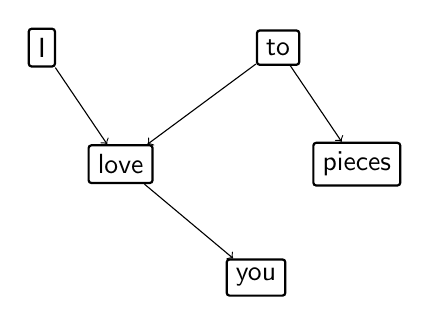
\begin{tikzpicture}[rotate=0,scale=4,font=\sffamily]

\definecolor{def_node_fill}{RGB}{255,255,255}
\definecolor{def_node_text}{RGB}{0,0,0}
\definecolor{def_node_draw}{RGB}{0,0,0}
\tikzstyle{default_node_style}=[draw=def_node_draw,fill=def_node_fill,text=def_node_text,line width = 0.8pt]

\definecolor{def_edge_draw}{RGB}{0,0,0}
\definecolor{def_edge_text}{RGB}{0,0,0}
\tikzstyle{default_edge_style}=[draw=def_edge_draw,text=def_edge_text, line width = 0.4pt]

\node(I) at (0.96,-2.28) [rectangle, rounded corners = 1,default_node_style] {I};

\node(love) at (1.21,-2.65) [rectangle, rounded corners = 1,default_node_style] {love};

\node(you) at (1.64,-3.01) [rectangle, rounded corners = 1,default_node_style] {you};

\node(to) at (1.71,-2.28) [rectangle, rounded corners = 1,default_node_style] {to};

\node(pieces) at (1.96,-2.65) [rectangle, rounded corners = 1,default_node_style] {pieces};

\draw[default_edge_style](I) edge node[above] {} (I);
\draw[default_edge_style](to) edge node[above] {} (to);
\draw[->,default_edge_style](I) edge node[above] {} (love);
\draw[->,default_edge_style](love) edge node[above] {} (you);
\draw[->,default_edge_style](to) edge node[above] {} (love);
\draw[->,default_edge_style](to) edge node[above] {} (pieces);

\end{tikzpicture}